\subsubsection{UC1 - Inserimento dati}
\begin{figure}[h]
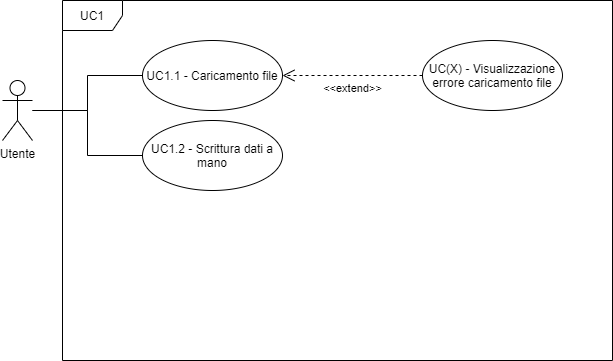
\includegraphics[width=\linewidth]{Section/Images/UC1InserimentoDati.png}
\centering
\caption{UC1 - Inserimento dati}
\end{figure}
\begin{itemize}
	\item \textbf{Attore primario}: Utente.
	\item \textbf{Precondizioni}: Il sistema è raggiungibile e funzionante.
	\item \textbf{Postcondizioni}: I dati sono stati inseriti nel database.
	\item \textbf{Scenario principale}:
		\begin{enumerate}
			\item L'utente seleziona "inserisci dati";
			\item L'utente può decidere se:
			\begin{enumerate}
			\item caricare un file contenente dati [UC1.1].
			\item scrivere i dati a mano [UC1.2].
			\end{enumerate}
		\end{enumerate}
	\item \textbf{Estensioni}:
\end{itemize}